%
%%%%%%%%%%%%%%%%%%%%%%%%%%%%%%%%%%%%%%%%%%%%%%%%%%%%%%%%%%%%%%%%%%%%%%%%%%

\documentclass[12pt,onecolumn,reqno]{amsart}
\usepackage{subcaption,wrapfig,graphicx,booktabs,fancyhdr,amsmath,amsfonts}
\usepackage{cite,bm,amssymb,amsthm,wasysym,url,multirow,float,mathtools,hyperref}
\usepackage{float}
\newcommand{\vb}{\boldsymbol}
\newcommand{\vbh}[1]{\hat{\boldsymbol{#1}}}
\newcommand{\vbb}[1]{\bar{\boldsymbol{#1}}}
\newcommand{\vbt}[1]{\tilde{\boldsymbol{#1}}}
\newcommand{\vbs}[1]{{\boldsymbol{#1}}^*}
\newcommand{\vbd}[1]{\dot{{\boldsymbol{#1}}}}
\newcommand{\by}{\times}
\newcommand{\tr}{{\rm tr}}
\newcommand{\sfrac}[2]{\textstyle \frac{#1}{#2}}
\newcommand{\ba}{\begin{array}}
\newcommand{\ea}{\end{array}}
\renewcommand{\earth}{\oplus}
\newcommand{\sinc}{{\rm sinc}}
\renewcommand{\equiv}{\triangleq}
\newcommand{\cnr}{C/N_0}
\newcommand{\sgn}{\rm sgn}
\renewcommand{\Re}{\mathbb{R}}
\renewcommand{\Im}{\mathbb{I}}
\newcommand{\E}[1]{\mathbb{E}\left[ #1 \right]}
\newcommand{\norm}[1]{\left\lVert#1\right\rVert}
\DeclareMathAlphabet{\mathpzc}{OT1}{pzc}{m}{it}

\topmargin = 0 mm 
\oddsidemargin = -1 mm 
\evensidemargin = -1 mm
\headheight = 0 mm 
\headsep = 8 mm 
\textheight = 220 mm 
\textwidth =170 mm 
\parindent = 0 mm
\parskip = 4 mm 

\setcounter{MaxMatrixCols}{15}

%%% ----------------------------------------------------------------------
\begin{document}
\title[]{Feedback Control Systems Final Report \\ Caravan Control}
\author[]{Tucker Haydon and Connor Brashar}
\address{The University of Texas at Austin}
\email{thaydon@utexas.edu, connor.brashar@utexas.edu}
\date{\today}
\begin{abstract}
  This is the project abstract.
\end{abstract}
\maketitle


%%% ----------------------------------------------------------------------
\section{Scenario}
You are an engineer in charge of designing and implementing an estimation and
control system for a fleet of self-driving semi-trucks. Due to government
regulation, the truck fleet can only operate in the self-driving mode when they
are on long, straight stretches of highway between cities. In order to reduce
costs and conserve fuel, the trucks drive very closely together at a
pre-determined speed in `caravan formation'. By driving very closely together,
the trucks can draft off of one another, reduce drag, and save fuel by upwards
of 21\% \cite{bonnet2000fuel}.

For the system you are designing, only three trucks will be in the caravan. The
caravan is equipped with the following sensor suite: 
\begin{enumerate}
  \item The lead truck is equipped with a GPS receiver that measures its
    position at 1 Hz.
  \item The two following trucks are equipped with range sensors that measure
    the relative position between themselves and the truck in front of them at
    10 Hz.
\end{enumerate}

Each truck may be independently controlled and may be instructed to either
accelerate or decelerate.

%%% ----------------------------------------------------------------------
\section{Nominal System Description}
\label{sec:nominal_system}

Define the system state.
\begin{equation}
  \vec{x} = 
  \begin{bmatrix}
    x_{1} \\
    x_{2} \\
    x_{3} \\
    v_{1} \\
    v_{2} \\
    v_{3}
  \end{bmatrix}
\end{equation}

Define the system input.
\begin{equation}
  \vec{u} = 
  \begin{bmatrix}
    a_{1} \\
    a_{2} \\
    a_{3}
  \end{bmatrix}
\end{equation}

Define the system dynamics.
\begin{equation}
  \dot{\vec{x}}
  =
  \begin{bmatrix}
    v_{1} \\
    v_{2} \\
    v_{3} \\
    a_{1} \\
    a_{2} \\
    a_{3}
  \end{bmatrix}
  =
  \underbrace{
  \begin{bmatrix}
    0 & 0 & 0 & 1 & 0 & 0  \\
    0 & 0 & 0 & 0 & 1 & 0  \\
    0 & 0 & 0 & 0 & 0 & 1  \\
    0 & 0 & 0 & 0 & 0 & 0  \\
    0 & 0 & 0 & 0 & 0 & 0  \\
    0 & 0 & 0 & 0 & 0 & 0  \\
  \end{bmatrix}
  }_{A}
  \vec{x}
  +
  \underbrace{
  \begin{bmatrix}
    0 & 0 & 0 \\
    0 & 0 & 0 \\
    0 & 0 & 0 \\
    1 & 0 & 0 \\
    0 & 1 & 0 \\
    0 & 0 & 1 \\
  \end{bmatrix}
  }_{B}
  \vec{u}
\end{equation}

Define the system observer equation.
\begin{equation}
  \vec{y} = 
  \begin{bmatrix}
    x_{1}             \\
    \Delta x_{12}     \\
    \Delta x_{23}     \\
    a_{1}             \\
    a_{2}             \\
    a_{3}             
  \end{bmatrix}
  =
  \underbrace{
  \begin{bmatrix}
    1 & 0 & 0 & 0 & 0 & 0   \\
    1 & -1 & 0 & 0 & 0 & 0  \\
    0 & 1 & -1 & 0 & 0 & 0  \\
    0 & 0 & 0 & 0 & 0 & 0   \\
    0 & 0 & 0 & 0 & 0 & 0   \\
    0 & 0 & 0 & 0 & 0 & 0  
  \end{bmatrix}
  }_{C}
  \vec{x}
\end{equation}

\subsection{Observability}
Using the nominal system, determine whether or not the system is observable. The
nominal system is linear and time-invariant, so the observability Grammian is
simplified:

\begin{equation}
  W_{o} = 
  \begin{bmatrix}
    C      \\
    CA     \\
    CA^2   \\
    \vdots \\
    CA^{n-1}
  \end{bmatrix}
\end{equation}

If the rank of $W_{o} = n$ then the system is observable. \textbf{The nominal
system is observable}.


\subsection{Controllability}
Using the nominal system, determine whether or not the system is controllable. The
nominal system is linear and time-invariant, so the controllability Grammian is
simplified:

\begin{equation}
  W_{c} = 
  \begin{bmatrix}
    B & AB & A^2B & \hdots & A^{n-1}N
  \end{bmatrix}
\end{equation}

If the rank of $W_{c} = n$ then the system is controllable. \textbf{The nominal
system is controllable}.

\subsection{Conclusion}
The fact that the nominal system is both observable and controllable indicates
that it is well-designed and amenable to both estimation and control.


%%% ----------------------------------------------------------------------
\section{Estimator} \label{sec:kalman_filter}

Estimators are designed to predict each state in a system, if that state
information is not directly observable. Often, measurements are taken that
contain indirect information about a state. For example, often accelerometer
measurements are used in navigation to take measurements of acceleration, which
can then be integrated twice to get position over time. Naturally, there is some
noise and inaccuracy in this process, but provided the system is fully
observable, a Kalman filter can be implemented on a linear system to get
observation of state variables from measurement data. 

Kalman filters are a simple form of estimator that works on linear systems of the form:

\begin{figure}[H]
	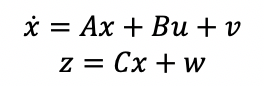
\includegraphics{system_eqs.png}
	\label{fig:Estimation System Equations}
\end{figure}

We note that the Kalman filter assumes no user input related to the measurement.
Because user input is fully known, we don't wish to include it in our states
that we are estimating. As a result, our Kalman Filter will not try to estimate
acceleration, only position and velocity. Otherwise, the Kalman filter model is
sufficient for this caravan problem.

A Kalman filter operates in two steps. 

\subsection{A Priori Measurements}
In the first, the kalman filter performs an `a priori' estimate, through which
it produces an estimate of the state at the current discrete time step based
only on the previous time step:

\begin{figure}[H]
	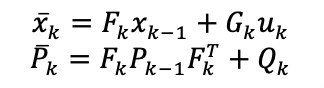
\includegraphics{a_priori.png}
	\label{fig:A Priori Estimate}
\end{figure}

Here, the P matrix is the covariance matrix of the system's states, while Q is a
measure of the system's state noise. Discrete-time process noise can be modeled
as follows:

\begin{figure}[H]
	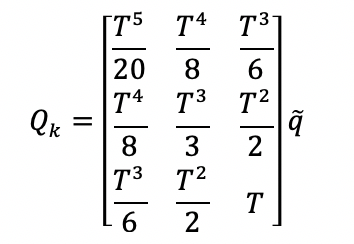
\includegraphics{Q.png}
	\label{fig:Q Matrix}
\end{figure}

Where T is the period between each measurement, here defined as 0.1s, and  is
the power spectral density (PSD) of noise for each component. For our system, we
used relatively low process noise with a PSD of 1/10 for position, and 1/20 for
velocity. We also note that the values of Fk and Gk are the discrete-time system
dynamics, which are covered in another section of this paper, rather than
continuous-time dynamics. 

\subsection{A Posteriori Measurements}
Next, the Kalman filter takes new measurements into the system and incorporates
them. The Kalman filter creates a model for measurements and compares it to the
actual measurement data it receives, and weights it's a priori estimate with the
new information to create a new, a posteriori measurement.

\begin{figure}[H]
	
\includegraphics{a_post.png}
	\label{fig:A Posteriori Measurements}
\end{figure}

The A posteriori formula can take many forms, and the form above is known as the
Joseph's form. The reason it is used in lieu of other forms is that the Joseph's
form equation copes well with sparse transition matrices that may lead to low
precision inversion of the $P_{zz}$ term. As a result, the Joseph's form works
best for this system, which has some very sparse matrices.

The final result, $\hat{x}$, is the most accurate version of the system states
based on both a model of how these states grow, and measurements that relate to
those states.

\subsection{Different Measurements at Different Times}
For our system, two measurements were taken: position of the first vehicle, and
range between each vehicle in the caravan. The former was taken once a second,
while the latter was taken ten times each second. As a result, we wish to
combine both measurements into the Kalman filter as these data come. How do we
accommodate this in our Kalman filter system' There are two ways to accommodate
measurements taken at different times in a Kalman filter: The first is to change
the measurement noise covariance matrix R such that it assumes an infinite
potential variance on measurement data for measurements that aren't present at
this time step. The other method is to have a varied-length measurement input Z,
and to change the size of the matrix Hk at each step depending on the size of
the Z vector. This latter method was chosen for this Kalman filter, as it worked
better for this implementation with the matrix sparcity as it was. In instances
where the Z vector didn't include the position measurement, the top row of the H
vector was clipped off.

%%% ----------------------------------------------------------------------
\section{Control System Description}
\subsection{Error State System}
Controllers drive systems to the origin. The nominal system, however, should not
be driven to the origin. Instead an error-state system should be specified where
the error is the deviation of the nominal system from a reference signal.

First, define the reference signal. From the problem statement, the goal is to
maintain a specified distance between the trucks and to keep that at a constant
velocity.
\begin{equation}
  \vec{x_{r}} = 
  \begin{bmatrix}
    x_{1_{r}}         \\
    \Delta x_{12_{r}} \\
    \Delta x_{23_{r}} \\
    v_{1_{r}}         \\
    v_{2_{r}}         \\
    v_{3_{r}}
  \end{bmatrix}
\end{equation}

The error signal is the difference between the nominal and the reference states.
Note that not all states have a corresponding reference signal.
\begin{equation}
  \vec{x_{e}} = 
  \begin{bmatrix}
    x_{1} - x_{2} - \Delta x_{12_{r}} \\
    x_{2} - x_{3} - \Delta x_{23_{r}} \\
    v_{1} - v_{1_{r}}
  \end{bmatrix}
\end{equation}

The error signal dynamics don't conform to the standard $\dot{x} = Ax + Bu$ form
--- there is an affine transform between the error dynamics and the nominal and
reference signals. However, the standard form can be composed via the following
trick: append the reference signal to the nominal state and define zero dynamics
and full observability for the reference substate.

Stack the nominal and reference states into the \textit{stacked state}.
\begin{equation}
  \vec{x_{s}} = 
  \begin{bmatrix}
    x_{1}             \\
    x_{2}             \\
    x_{3}             \\
    v_{1}             \\
    v_{2}             \\
    v_{3}             \\ 
    \Delta x_{12_{r}} \\
    \Delta x_{23_{r}} \\
    v_{1_{r}}
  \end{bmatrix}
\end{equation}

Define the stacked state dynamics.
\begin{equation}
  \dot{\vec{x}}_{s} = 
  \begin{bmatrix}
    v_{1}             \\
    v_{2}             \\
    v_{3}             \\
    a_{1}             \\
    a_{2}             \\
    a_{3}             \\ 
    0                 \\
    0                 \\
    0
  \end{bmatrix}
  =
  \underbrace{
  \begin{bmatrix}
    0 & 0 & 0 & 1 & 0 & 0 & 0 & 0 & 0 & 0 & 0 \\
    0 & 0 & 0 & 0 & 1 & 0 & 0 & 0 & 0 & 0 & 0 \\
    0 & 0 & 0 & 0 & 0 & 1 & 0 & 0 & 0 & 0 & 0 \\
    0 & 0 & 0 & 0 & 0 & 0 & 0 & 0 & 0 & 0 & 0 \\
    0 & 0 & 0 & 0 & 0 & 0 & 0 & 0 & 0 & 0 & 0 \\
    0 & 0 & 0 & 0 & 0 & 0 & 0 & 0 & 0 & 0 & 0 \\
    0 & 0 & 0 & 0 & 0 & 0 & 0 & 0 & 0 & 0 & 0 \\
    0 & 0 & 0 & 0 & 0 & 0 & 0 & 0 & 0 & 0 & 0 \\
    0 & 0 & 0 & 0 & 0 & 0 & 0 & 0 & 0 & 0 & 0
  \end{bmatrix}
  }_{A_{s}}
  \vec{x}_{s}
  +
  \underbrace{
  \begin{bmatrix}
    0 & 0 & 0 \\
    0 & 0 & 0 \\
    0 & 0 & 0 \\
    1 & 0 & 0 \\
    0 & 1 & 0 \\
    0 & 0 & 1 \\
    0 & 0 & 0 \\
    0 & 0 & 0 \\
    0 & 0 & 0
  \end{bmatrix}
  }_{B_{s}}
  \vec{u}
\end{equation}

Define the stacked state observer equation. Note that the reference states are
specified and fully known so there is full state feedback for these states.
\begin{equation}
  \vec{y} = 
  \begin{bmatrix}
    x_{1}             \\
    \Delta x_{12}     \\
    \Delta x_{23}     \\
    a_{1}             \\
    a_{2}             \\
    a_{3}             \\
    \Delta x_{12_{r}} \\
    \Delta x_{23_{r}} \\
    v_{1_{r}}
  \end{bmatrix}
  =
  \underbrace{
  \begin{bmatrix}
    1 & 0 & 0 & 0 & 0 & 0 & 0 & 0 & 0 & 0 & 0 & 0 \\
    1 & -1 & 0 & 0 & 0 & 0 & 0 & 0 & 0 & 0 & 0 & 0 \\
    0 & 1 & -1 & 0 & 0 & 0 & 0 & 0 & 0 & 0 & 0 & 0 \\
    0 & 0 & 0 & 0 & 0 & 0 & 0 & 0 & 0 & 0 & 0 & 0 \\
    0 & 0 & 0 & 0 & 0 & 0 & 0 & 0 & 0 & 0 & 0 & 0 \\
    0 & 0 & 0 & 0 & 0 & 0 & 0 & 0 & 0 & 0 & 0 & 0 \\
    0 & 0 & 0 & 0 & 0 & 0 & 0 & 0 & 0 & 1 & 0 & 0 \\
    0 & 0 & 0 & 0 & 0 & 0 & 0 & 0 & 0 & 0 & 1 & 0 \\
    0 & 0 & 0 & 0 & 0 & 0 & 0 & 0 & 0 & 0 & 0 & 1 \\
  \end{bmatrix}
  }_{C_{s}}
  \vec{x}_{s}
  +
  \underbrace{
  \begin{bmatrix}
    0 & 0 & 0 \\
    0 & 0 & 0 \\
    0 & 0 & 0 \\
    1 & 0 & 0 \\
    0 & 1 & 0 \\
    0 & 0 & 1 \\
    0 & 0 & 0 \\
    0 & 0 & 0 \\
    0 & 0 & 0
  \end{bmatrix}
  }_{D_{s}}
  \vec{u}
\end{equation}

Now define the error state by linearly transforming the stacked state via a
\textit{similiarity transform}.

\begin{equation*}
  \vec{x}_{e} = 
  \begin{bmatrix}
    x_{1}               \\
    \Delta x_{12_{e}}   \\
    \Delta x_{23_{e}}   \\
    v_{1_{e}}           \\
    v_{2}               \\
    v_{3}               \\ 
    \Delta x_{12_{r}}   \\
    \Delta x_{23_{r}}   \\
    v_{1_{r}}
  \end{bmatrix}
  =
  \underbrace{
  \begin{bmatrix}
    1 & 0 & 0 & 0 & 0 & 0 & 0 & 0 & 0 \\
    1 & -1 & 0 & 0 & 0 & 0 & -1 & 0 & 0 \\
    0 & 1 & -1 & 0 & 0 & 0 & 0 & -1 & 0 \\
    0 & 0 & 0 & 1 & 0 & 0 & 0 & 0 & -1 \\
    0 & 0 & 0 & 0 & 1 & 0 & 0 & 0 & 0 \\
    0 & 0 & 0 & 0 & 0 & 1 & 0 & 0 & 0 \\
    0 & 0 & 0 & 0 & 0 & 0 & 1 & 0 & 0 \\
    0 & 0 & 0 & 0 & 0 & 0 & 0 & 1 & 0 \\
    0 & 0 & 0 & 0 & 0 & 0 & 0 & 0 & 1
  \end{bmatrix}
  }_{T}
  \begin{bmatrix}
    x_{1}             \\
    x_{2}             \\
    x_{3}             \\
    v_{1}             \\
    v_{2}             \\
    v_{3}             \\ 
    \Delta x_{12_{r}} \\
    \Delta x_{23_{r}} \\
    v_{1_{r}}
  \end{bmatrix}
\end{equation*}

Now, leverage the similarity transform to define the error state dynamics.
\begin{align*}
  \dot{\vec{x}}_{e} &= T A_{s} T^{-1} \vec{x}_{e} + T B_{s} \vec{u} \\
  y &= C T^{-1} \vec{x}_{e} + D \vec{u}
\end{align*}

Finally, clean up the equation by redefining the system.
\begin{align*}
  \vec{x} &\coloneqq \vec{x}_{e}    \\
  A       &\coloneqq T A_{s} T^{-1} \\
  B       &\coloneqq T B_{s}        \\
  C       &\coloneqq C_{s} T^{-1}   \\
  D       &\coloneqq D
\end{align*}

Now the system is in the standard form.
\begin{align*}
  \dot{\vec{x}} &= A \vec{x} + B \vec{u} \\
  y &= C \vec{x} + D \vec{u}
\end{align*}


\subsection{Discrete-Time Dynamics}
Software implementations of continuous kinematic systems must first discretize
the system dynamics. Many sensors and computers cannot produce nor consume
continuous signals. As a result, system dynamics or measurements are
represented as discrete systems. 

Define the discrete system. 
\begin{align*}
  x_{k+1} = A_{d} x_{k} + B_{d} u_k \\
  y_{k} = C x_{k} + D u_{k}
\end{align*}

For a discretized system, only the system dynamics matrices (A, B) change:
\begin{align*}
  A_{d} = e^{A \cdot \Delta T} \\
  B_d = \int_{0}^{\Delta T} e^{A \lambda} d \lambda B
\end{align*}
where $\Delta T$ is the discrete time interval. For this project, $\Delta T$ was
chosen to match the smallest measurement interval, $\Delta T = 0.1$.


\subsection{Discrete-Time, Finite Horizon LQR Controller}
A discrete-time, finite horizon LQR controller was chosen to bring the trucks
into `caravan' formation. Given a transient state weighting matrix, $Q$, a final
state weighting matrix, $Q_{f}$, and an input weighting matrix, $R$, LQR
controllers minimize the cost function:
\begin{equation*}
  J = \vec{x}_{f}^{T} Q_{f} \vec{x}_{f} + \sum_{k=0}^{N} \left[ \vec{x}_{k}^{T} Q
  \vec{x}_{k} + \vec{u}_{k}^{T} R \vec{u}_{k} \right]
\end{equation*}

Together, the Kalman Filter described in section \ref{sec:kalman_filter} and the
LQR controller described in this section form a Linear-Quadratic-Gaussian
controller.


%%% ----------------------------------------------------------------------
\section{Simulation}
The LQG controller was implemented in Matlab. The goal of the controller is to
bring the trucks into the 'caravan' formation within 10 minutes. The trucks
should follow each other at 30 meters/second with a separation of only 5 meters.

\begin{equation*}
  \vec{x}_{r} = 
  \begin{bmatrix}
    \Delta x_{12} \\ 
    \Delta x_{23} \\ 
    v_{1}
  \end{bmatrix} 
  =
  \begin{bmatrix}
    5 \\
    5 \\
    30
  \end{bmatrix} 
\end{equation*}

\begin{figure}[H]
	\includegraphics[width=\linewidth]{state_error_over_time_with_truth.jpg}
	\caption{Tracking Error with True State}
	\label{fig:Tracking Error with True State}
\end{figure}

\begin{figure}[H]
	\includegraphics[width=\linewidth]{state_error_over_time.jpg}
	\caption{Tracking Error with Estimated State}
	\label{fig:Tracking Error with Kalman Filter}
\end{figure}


%%% ----------------------------------------------------------------------
\section{Discussion}
The LQG 

\subsection{Kalman Filter}
The Kalman filter was run both with and without control input to ensure that it
was working. In both cases, the filter's error between estimated state and true
state was driven to zero within two minutes. A plot of the estimation error and
variances of estimated state positions is given below. 

\begin{figure}[H]
	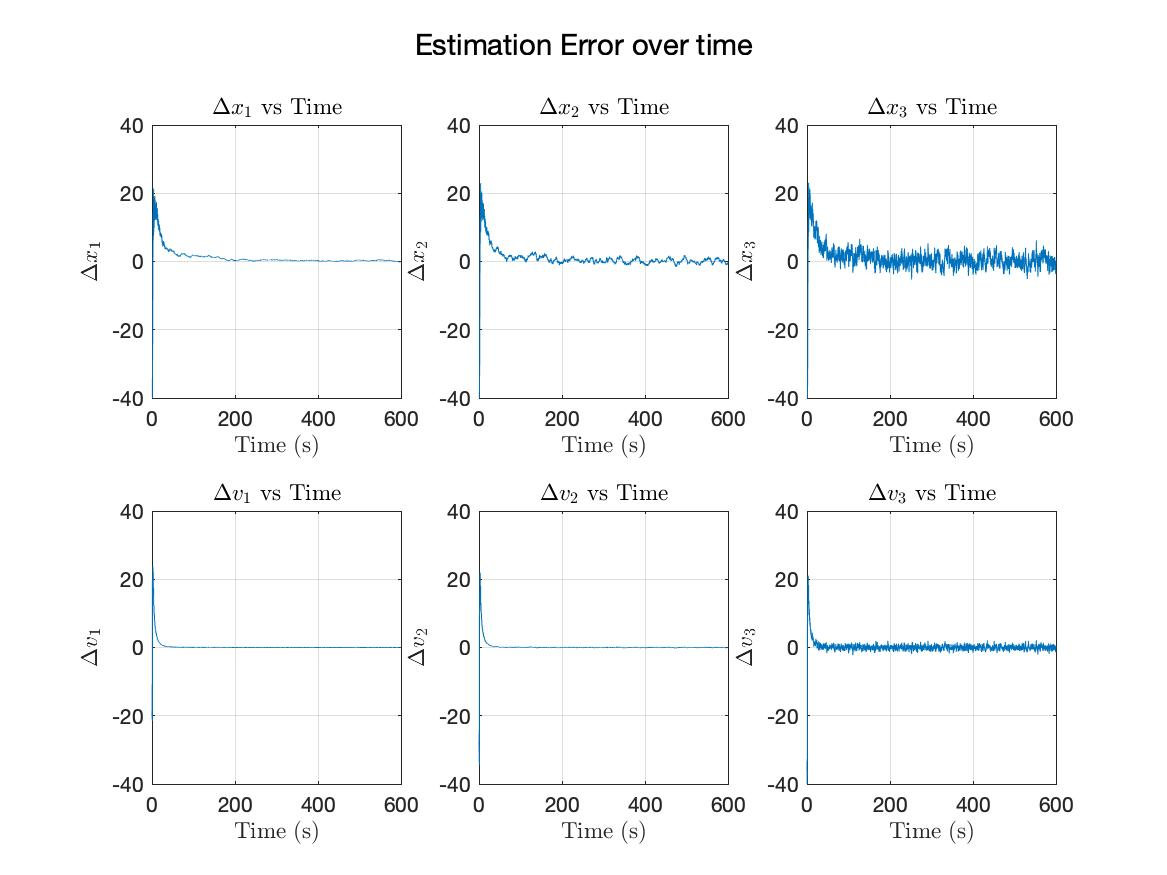
\includegraphics[width=\linewidth]{estimation_error_over_time.jpg}
	\caption{Estimation Error}
	\label{fig:Est. Error}
\end{figure}

\begin{figure}[H]
	\includegraphics[width=\linewidth]{estimation_variances_over_time.jpg}
	\caption{Estimated State Variances}
	\label{fig:Est. State Vars}
\end{figure}

As can be seen, the estimation error is driven to zero quickly, and remains
relatively stable throughout the system. In a few rare instances, a noisy
measurement of vehicle position bounced the error up for a second or two, but
these errors were quickly accommodated by the Kalman filter.

The error of each state was interesting. The kalman filter trusted its estimate
of each vehicle position in the caravan less than the vehicle in front of it.
This makes sense, given that only the first vehicle has actual position
measurements, and subsequent position estimates have more and more noise (driven
by range values). This intuitive image of how the Kalman Filter was able to
estimate vehicle positions and velocities helped to confirm that the Kalman
filter was operating exactly as expected.


%%% ----------------------------------------------------------------------
\section{Museum Exhibit}
The following section describes a potential museum exhibit aimed at high-school
and middle-school children.

Note that this section is an abridged version of the original project proposal.
In discussion with Dr. Tanaka, we agreed that the primary portion of the project
would be the design, implementation, and simulation of an LQG controller and
that, to make grading easier, we would try to conform to the original project
proposal.

\subsection{Description}
We propose a museum exhibit composed of toy trains on tracks where visitors
attempt to tune an LQR controller to bring three independent locomotives into
the caravan formation. On a 3 meter by 3 meter tables, toy train tracks are laid
out in a wide circle \footnote {The hope is that a wide circle will
approximately represent a long, straight, endless track}. Three battery-powered
locomotives may be placed anywhere on the tracks. Visitors may turn 6 knobs
corresponding to the 6 diagonal entries of the LQR weighting matrices to tune
the system.


\subsection{Implementation}
Visitors may walk around all sides of the table. On one side of the table are
six knobs that visitors may twist to tune the LQR controller. On the far end of
the table opposite the knobs is a TV. The TV first shows a short 30-second video
describing the goal of the exhibit, what a 'good' controller looks like, and
what each of the 6 knobs do. Visitors are then free to twist the knobs (a
digital value is displayed on the screen), and then press the 'go' button.

Behind the scenes, a Raspberry Pi B+ (RPB) controls the three locomotives. The
locomotives have been 'hacked' and carry a Raspberry Pi Zero (RPZ) that
modulates the supplied battery voltage to each of the locomotives. By modulating
the battery voltage, the RPZ can directly control the speed of each of the
locomotives. Each of the RPZs carry an inertial measurement unit that measures
the acceleration of each of the locomotives. The RPZs transmit the acceleration
data to the RPB via wifi. A camera is suspended above the table and connected to
the RPB. The RPB uses an image processing algorithm on the incoming camera data
to track the location of each of the locomotives and generate the position and
position difference measurements. The RPB fuses the camera measurements and the
accelerometer measurements together with the kalman filter described in section
\ref{sec:kalman_filter}.

After the 'go' button is pressed, the RPB reads in the current analog knob
values and solves the discrete-time algebraic riccati equation. Once solved, the
RPB streams control input commands to the RPZs via wifi. The RPZs convert the
control input into motor voltages and drive the locomotives. 

If the camera detects that two locomotives have touched (i.e. a crash has
occurred), the trains are stopped, and the visitor is notified of the crash and
given another chance.


\subsection{Price Breakdown}
\begin{center}
  \begin{tabular} { || l c || }
    \hline
    Item & Total Price \\ [0.5ex] 
    \hline\hline
    2 Wooden Train Track          & \$100 \\
    3 Battery-Powered Locomotives & \$150 \\
    1 Raspberry Pi B+             & \$40  \\
    1 Wifi Dongle                 & \$15  \\
    1 Raspberry Pi Camera Module  & \$25  \\
    3 Raspberry Pi Zero W         & \$30  \\
    3 IMU Sensors                 & \$45  \\
    3 PWM Motor Shields           & \$120  \\
    1 LCD TV                      & \$300 \\ 
    6 Knobs and 1 button          & \$50  \\
    \hline
    Total Price                   & \$875 \\
    \hline
  \end{tabular}
\end{center}

\section{Work Contribution}
Both Connor Brashar and Tucker Haydon contributed equally to this project.


%%% ----------------------------------------------------------------------
\bibliographystyle{ieeetr}
\bibliography{report.bib}
\end{document}


